\documentclass[10pt,twocolumn]{article}

%\usepackage{draftwatermark}
%\SetWatermarkText{arXiv Preprint}
%\SetWatermarkScale{1.5}
%\SetWatermarkLightness{0.9}

% ---------- Layout & fonts ----------
\usepackage[letterpaper,margin=1in]{geometry}
\setlength{\columnsep}{0.28in}
\usepackage{microtype}
\usepackage{lmodern}
\usepackage[T1]{fontenc}
\usepackage[utf8]{inputenc}
\usepackage{placeins}
\usepackage{needspace}
\usepackage{stfloats}
\usepackage{inconsolata}
\usepackage{dirtree}
\usepackage{setspace}
\usepackage{enumitem}

% ---------- Math & symbols ----------
\usepackage{amsmath,amssymb,amsfonts,mathtools}
\usepackage{bbm}

% ---------- Graphics & floats ----------
\usepackage{graphicx}
\graphicspath{{figures/}}
\usepackage[font=small,labelfont=bf]{caption}
\usepackage{subcaption}
\usepackage{booktabs}
\usepackage{float}

% ---------- TikZ ----------
\usepackage{tikz}
\usetikzlibrary{arrows.meta,positioning,fit,calc,shapes,backgrounds}
\tikzset{
  box/.style={draw, rounded corners, thick, align=center, inner sep=6pt, fill=gray!5},
  bigbox/.style={draw, rounded corners, ultra thick, align=center, inner sep=8pt, fill=gray!3},
  head/.style={draw, rounded corners, thick, align=center, inner sep=4pt, fill=blue!6},
  enc/.style={draw, rounded corners, thick, align=center, inner sep=4pt, fill=green!6},
  bias/.style={draw, rounded corners, thick, align=center, inner sep=3pt, fill=orange!15},
  loss/.style={draw, rounded corners, thick, align=center, inner sep=3pt, fill=red!8},
  arrow/.style={-Latex, thick},
  dashedarrow/.style={-Latex, thick, dashed},
}

% Tighter float spacing
\setlength{\textfloatsep}{8pt plus 2pt minus 2pt}
\setlength{\floatsep}{8pt plus 2pt minus 2pt}
\setlength{\intextsep}{8pt plus 2pt minus 2pt}
\setlength{\dbltextfloatsep}{8pt plus 2pt minus 2pt}
\setlength{\dblfloatsep}{8pt plus 2pt minus 2pt}

% ---------- Citations ----------
\usepackage[numbers,sort&compress]{natbib}

% ---------- TOC ----------
\usepackage{multicol}
\usepackage{tocloft} 
\usepackage{etoolbox}  

% ---------- Links & clean references ----------
\usepackage{xcolor}
\usepackage[colorlinks=true,linkcolor=black,citecolor=black,urlcolor=blue]{hyperref}
\usepackage[capitalize,noabbrev]{cleveref}

% ---------- Algorithms ----------
\usepackage{algorithm}
\usepackage{algpseudocode}

% ---------- Title / authors ----------
\usepackage{authblk}
\title{\textbf{\emph{It\^oFormer}: Augmenting Stochastic Validity in Financial-Centric Deep Neural Networks}}

\author{
{\Large \textbf{Nathaniel Coulter}$^{1}$}\thanks{%
  \href{mailto:nathaniel.coulter21@my.stjohns.edu}{\texttt{\textcolor{blue}{nathaniel.coulter21@my.stjohns.edu}}}\\
  \href{https://github.com/Nathaniel-Coulter}{\texttt{\textcolor{blue}{https://github.com/Nathaniel-Coulter}}}%
}
\vspace{-0.5em} \\ 
\small $^{1}$\textbf{Department of Mathematics and Computer Science,\\ \textit{St.~John's University, NY}}
}
\date{}

% ---------- Useful macros ----------
\newcommand{\E}{\mathbb{E}}
\newcommand{\Var}{\mathrm{Var}}
\newcommand{\R}{\mathbb{R}}
\newcommand{\model}{\textsc{PatchTST}}
\newcommand{\ours}{\textsc{Cross-Lite}}

\begin{document}
\maketitle
\begin{abstract}
This study proposes \emph{It\^oFormer}, a finance-native transformer architecture rooted in It\^o Calculus\cite{ito1944stochastic}, that enforces
stochastic validity within attention-based\cite{vaswani2017attention} sequence models. Unlike standard calculus, which deals with smooth and predictable functions; \emph{It\^o's Lemma} 
extends the chain rule to account for the non-zero quadratic variation of random processes encountered in stochastic differential equations\cite{oksendal2003sde}. \\

While transformers have achieved state-of-the-art results in NLP and vision, our previous work has shown that vanilla architectures do not map cleanly onto financial time series, which are inherently stochastic and non-stationary\cite{coulter2025tokenization,coulter2025neural}. These limitations arise from mismatched design assumptions, such as deterministic sequence mappings, lack of variance modeling, and weak treatment of temporal causality. \\

To address this gap, \emph{It\^oFormer} integrates domain-specific inductive biases inspired by stochastic calculus: quadratic variation-aware attention, martingale consistency constraints, and no-arbitrage penalties for options and rates. We evaluate It\^oFormer across equities, fixed income, derivatives, and commodities, benchmarking against leading transformer variants from our previous works, such as: PatchTST, iTransformer, Crossformer, Autoformer, Fedformer, Informer, TimesNet, and TimeXer. Our results demonstrate that It\^oFormer reduces forecast error, improves hedging stability, and enforces structural consistency absent from prior architectures. 
For an in depth comparison between each of the afformentioned architectures, see: \textit{"Tokenization and Transformer Architectures for Cross-Asset Allocation: Controlled Ablation in Financial Time Series\cite{coulter2025tokenization}}.
\end{abstract}

\begin{minipage}[t]{0.48\textwidth}
  \renewcommand{\contentsname}{Contents}
  \setcounter{tocdepth}{2}
  \small
  \vspace*{-0.5em}
  \tableofcontents
\end{minipage}



\clearpage
\section*{Introduction}

The rise of transformer architectures has reshaped machine learning in natural language processing, computer vision, and increasingly, time series modeling. Yet, financial markets present unique challenges that distinguish them from language or vision domains: asset returns evolve as stochastic processes, exhibit structural breaks, and obey constraints such as no-arbitrage conditions. Standard architectures, designed for deterministic mappings, are often ill-suited for these properties.\\ 

Our earlier work has explored both neural and econometric approaches to this problem. In \textit{Neural Portfolio Allocators} \cite{coulter2025neural}, we tested reinforcement learning with Tsallis entropy and multi-agent transformer heads, alongside stochastic models such as MGARCH and Monte Carlo simulation. In \textit{Tokenization and Transformer Architectures for Cross-Asset Allocation} \cite{coulter2025tokenization}, we benchmarked nine modern transformer variants across equities, fixed income, and derivatives, highlighting their strengths but also their shared limitations when applied to stochastic financial series.\\

These studies converge on a central insight: vanilla transformer designs implicitly assume \textit{deterministic sequence-to-sequence mappings}, while financial time series demand models that respect stochastic validity. The mismatch manifests in several ways:

\begin{enumerate}
    \item \textbf{Deterministic vs. stochastic mappings:} Transformers excel in contexts where the future is conditionally deterministic (e.g., predicting the next word), but financial increments follow distributions, not fixed outcomes.
    \item \textbf{Stationarity and ergodicity:} Market data is often heteroskedastic and regime-shifting, violating assumptions of stable statistical structure.
    \item \textbf{Linearity of attention:} The softmax-weighted averaging in attention captures correlations but cannot encode stochastic dynamics such as variance evolution or jump processes.
    \item \textbf{Uncertainty modeling:} Standard architectures return point predictions, while finance requires modeling the full conditional distribution (expectation, variance, skew, and tails).
    \item \textbf{Temporal continuity and causality:} Markets evolve under stochastic differential equations, with increments scaling with $\sqrt{\Delta t}$; traditional attention layers lack this awareness.
\end{enumerate}

To address these incompatibilities, we propose \emph{It\^oFormer}, a finance-native transformer architecture that embeds inductive biases from stochastic calculus. By integrating Itô’s Lemma, martingale-consistency constraints, and quadratic variation awareness into the attention mechanism, It\^oFormer enforces structural validity while maintaining the flexibility of modern deep learning. 

This paper makes three primary contributions:
\begin{itemize}
    \item \textbf{Architecture:} We design the It\^oFormer block, which extends self-attention with stochastic calculus priors and penalty terms that align outputs with financial dynamics.
    \item \textbf{Cross-asset evaluation:} We test It\^oFormer across equities, fixed income, and derivatives, including volatility surfaces and option Greeks, benchmarking against state-of-the-art transformer variants.
    \item \textbf{Stochastic robustness:} We demonstrate improvements in forecast accuracy, hedging error stability, and structural consistency compared to both econometric baselines and prior neural approaches.
\end{itemize}

\section{It\^o Calculus: A Primer}

Classical calculus relies on differentiable functions and smooth changes. 
However, financial time series are inherently noisy, often modeled as stochastic processes driven by Brownian motion. 
In such settings, the rules of ordinary calculus no longer apply because increments are nowhere differentiable and exhibit non-zero \emph{quadratic variation}. 
It\^o calculus \cite{ito1944stochastic,oksendal2003sde} is the branch of stochastic calculus designed to handle precisely this regime. 
It provides the mathematical foundation for modern quantitative finance, option pricing, and stochastic modeling.

\subsection{From Classical Chain Rule to It\^o's Lemma}

In ordinary calculus, for a differentiable function $f(x,t)$, the chain rule reads:
\[
dz = f'(x) \, dx.
\]

But in stochastic calculus, increments like Brownian motion $W_t$ satisfy
\[
(dW_t)^2 = dt,
\]
meaning the quadratic variation does not vanish. This forces us to include second-order terms when applying Taylor expansions.\\ 

Suppose $X_t$ follows a stochastic differential equation (SDE):
\[
dX_t = \mu(X_t,t)\,dt + \sigma(X_t,t)\, dW_t,
\]
and let $f(X_t,t)$ be twice differentiable. By Taylor expanding,
\[
df = f_t\, dt + f_x\, dX_t + \tfrac{1}{2} f_{xx} (dX_t)^2 + o(dt).
\]

Substituting for $dX_t$ and applying It\^o's rules:
\[
(dt)^2 = 0, \quad dt \cdot dW_t = 0, \quad (dW_t)^2 = dt,
\]
we obtain
\[
(dX_t)^2 = \sigma^2\, dt.
\]

Thus,
\[
df = \Big(f_t + \mu f_x + \tfrac{1}{2}\sigma^2 f_{xx}\Big)\, dt + \sigma f_x\, dW_t.
\]

This is \textbf{It\^o's Lemma}, the stochastic extension of the chain rule. The additional 
$\tfrac{1}{2} f_{xx}\sigma^2 dt$ is the \emph{convexity correction} absent from ordinary calculus. 
It ensures stochastic models correctly capture variance effects and convex payoffs (e.g., option pricing).

\subsection{Step-by-Step Derivation of the It\^o Correction}

To see how the $\tfrac{1}{2} f_{xx}\sigma^2 dt$ term arises, consider the expansion:

\begin{align*}
f(X_{t+\Delta t},t+\Delta t) - f(X_t,t) 
&= f_t \Delta t + f_x \Delta X_t \\[-2pt]
&\quad + \tfrac{1}{2} f_{xx} (\Delta X_t)^2 + r_t,
\end{align*}

where $r_t$ is a remainder. Substituting $\Delta X_t = \mu \Delta t + \sigma \Delta W_t$, we have:

\[
(\Delta X_t)^2 = \mu^2 (\Delta t)^2 + 2\mu\sigma (\Delta t)(\Delta W_t) + \sigma^2 (\Delta W_t)^2.
\]

As $\Delta t \to 0$, the first two terms vanish in probability, while 
\[
(\Delta W_t)^2 \sim \Delta t.
\]

Thus,
\[
(\Delta X_t)^2 \to \sigma^2 \Delta t.
\]

Taking limits,
\[
df = f_t\, dt + f_x (\mu dt + \sigma dW_t) + \tfrac{1}{2} f_{xx}\, \sigma^2 dt.
\]

This establishes the It\^o correction.

\subsection{Brownian Motion and Quadratic Variation}

Brownian motion $W_t$ is a Gaussian process with independent increments:
\[
W_t - W_s \sim \mathcal{N}(0, t-s).
\]

Unlike smooth functions, its paths are continuous but nowhere differentiable. 
The variance of increments grows linearly with time, leading to:
\[
[dW_t]^2 = dt.
\]

This quadratic variation is the key departure from classical calculus, forcing us to adopt It\^o's rules.

\subsection{Martingales and Risk-Neutral Pricing}

It\^o integrals are constructed to preserve the martingale property:
\[
\mathbb{E}\left[\int_0^t \phi_s\, dW_s \mid \mathcal{F}_u\right] = 0, \quad u<t.
\]

Martingales formalize the “fair game” property of financial markets under no-arbitrage assumptions. 
The Doob–Meyer decomposition shows that semimartingales can be written as a martingale plus a finite-variation process, which underlies risk-neutral pricing. 
This connection is why It\^o calculus is inseparable from modern finance.

\subsection{Why It\^o, Not Stratonovich, Malliavin, or Rough Paths?}

Stochastic calculus is an umbrella framework including several variants:

\begin{itemize}
    \item \textbf{Stratonovich calculus} preserves the classical chain rule (no $\tfrac{1}{2}\sigma^2 f_{xx}$ term). It is well suited for physical SDEs with smooth noise, but not for finance, since trading strategies must be \emph{non-anticipative} and predictable. Convexity corrections are essential in pricing and hedging, making It\^o the natural choice.
    \item \textbf{Malliavin calculus} provides tools for pathwise derivatives and sensitivity analysis (e.g., Greeks). It is powerful for Monte Carlo gradient estimation, but it is not the core inductive bias we want in a sequence model. Instead, we can borrow its ideas for specific gradient estimators.
    \item \textbf{Rough paths theory} extends stochastic calculus to highly irregular signals, controlling pathwise behavior beyond Brownian motion. While promising, it is overly general for our financial setting and computationally burdensome.
\end{itemize}

In short, It\^o calculus is the discrete-time limit of predictable, adapted strategies with quadratic variation, and perfectly matched for trading in modern financial markets. 
Its correction term enforces convexity consistency, and its martingale structure aligns with no-arbitrage pricing. 
For these reasons, It\^o forms the mathematical backbone of our proposed architecture.

\subsection{Implications for Neural Networks \& Machine Learning}

Embedding It\^o principles into neural architectures ensures stochastic validity. In particular:

\begin{itemize}
    \item The quadratic-variation term corresponds to curvature risk, which our model must respect.
    \item Martingale-consistent heads enforce risk-neutral valuation and no-arbitrage.
    \item Attention mechanisms can be biased by predictable covariance structures, reflecting It\^o’s adapted integrands.
    \item Convexity-correction consistency ensures nonlinear feature maps (e.g., log, squares, option payoffs) remain stable under volatility regime shifts.
    \item Jump-aware dynamics incorporate It\^o--L\'evy terms, enabling robustness to discontinuities such as earnings gaps or macro shocks.\footnote{In this context, ``jump-aware'' refers to extending It\^o calculus with Poisson-driven components (It\^o--L\'evy processes), which capture sudden, discrete movements in asset prices rather than continuous Brownian motion.}
    \item Measure-consistency via Girsanov-inspired controls separates real-world alpha (P-world drift) from risk-neutral pricing and hedging (Q-world martingale).
\end{itemize}

These inductive biases turn transformers into finance-native architectures. 
Their impact is amplified when paired with complementary methods we detail later: econometric baselines for rigor, OOS walk-forward 
validation for robustness, and diagnostics such as sensitivity analysis and attention maps with compact RL executors and regime-aware encoders.

\section{It\^oFormer Architecture}

\subsection{Attention: Domain-Aware Biases}

At the core of It\^oFormer is a causal multi-head attention mechanism augmented with 
finance-native inductive biases:

\begin{itemize}
    \item \textbf{Time-decay bias:} recent information is weighted more heavily:
    \[
    B^{(\text{time})}_{ij} = -\lambda \,(t_i - t_j)_{+}.
    \]

    \item \textbf{Factor-correlation bias:} assets with shared factors are pulled closer:
    \[
    B^{(\text{corr})}_{ij} = \gamma \,\rho_{ij},
    \]
    where $\rho_{ij}$ is a rolling correlation (Kendall/Pearson or learned).

    \item \textbf{Martingale (risk-neutral) bias:} attention is centered on conditional expectation 
    under the risk-neutral measure $\mathbb Q$:
    \[
    B^{(\text{mart})}_{ij} = \mu \,\mathbf 1\{ j < i \},
    \]
    with strength modulated by a drift proxy.

    \item \textbf{Graph mask:} optional sparsity constraints induced by sector or curve topology.
\end{itemize}


The scaled dot-product attention then becomes:
\begin{equation}
\begin{aligned}
\text{Attn}(Q,K,V) &= \text{softmax}\!\Bigg(
    \frac{QK^\top}{\sqrt{d}} 
    + B^{(\text{time})} \\
    &\quad + B^{(\text{corr})} 
    + B^{(\text{mart})} 
    + M_{\text{graph}}
\Bigg)V,
\end{aligned}
\end{equation}
with a strict causal mask ensuring no leakage of future information.
Efficiency enhancements include FlashAttention and optional block-sparsity 
by curve or sector.
%------------------------------------------Ito attention biases (tikz)---------------------------------------------------------------
\begin{figure}[H]
\centering
\resizebox{\columnwidth}{!}{%
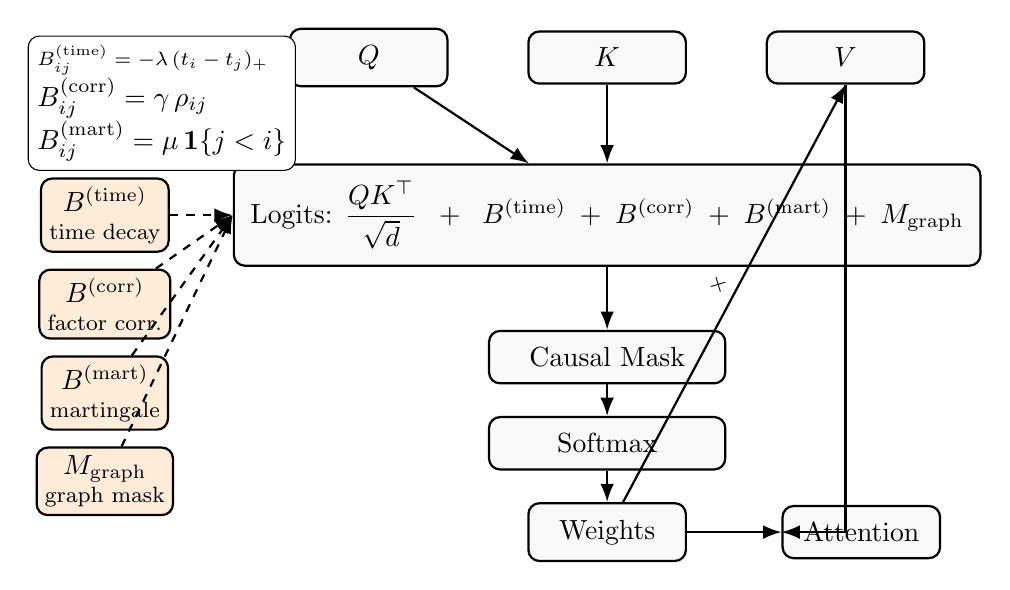
\begin{tikzpicture}[node distance=6mm and 8mm]
  % Q K V
  \node[box, minimum width=20mm] (Q) {$Q$};
  \node[box, right=10mm of Q, minimum width=20mm] (K) {$K$};
  \node[box, right=10mm of K, minimum width=20mm] (V) {$V$};

  % logits
  \node[box, below=10mm of K, minimum width=66mm, align=left] (logit) {%
    Logits: $\dfrac{QK^\top}{\sqrt d} \;\;+\;\; B^{(\text{time})} \;+\; B^{(\text{corr})} \;+\; B^{(\text{mart})} \;+\; M_{\text{graph}}$};

  \draw[arrow] (Q) -- (logit);
  \draw[arrow] (K) -- (logit);

  % biases side
  \node[bias, left=8mm of logit, align=center] (btime) {$B^{(\text{time})}$\\[-2pt]\footnotesize time decay};
  \node[bias, below=2mm of btime, align=center] (bcorr) {$B^{(\text{corr})}$\\[-2pt]\footnotesize factor corr.};
  \node[bias, below=2mm of bcorr, align=center] (bmart) {$B^{(\text{mart})}$\\[-2pt]\footnotesize martingale};
  \node[bias, below=2mm of bmart, align=center] (bgraph) {$M_{\text{graph}}$\\[-2pt]\footnotesize graph mask};

  \draw[dashedarrow] (btime) -- (logit.west);
  \draw[dashedarrow] (bcorr) -- (logit.west);
  \draw[dashedarrow] (bmart) -- (logit.west);
  \draw[dashedarrow] (bgraph) -- (logit.west);

  % softmax + mask
  \node[box, below=8mm of logit, minimum width=30mm] (mask) {Causal Mask};
  \node[box, below=4mm of mask, minimum width=30mm] (softmax) {Softmax};
  \node[box, below=4mm of softmax, minimum width=20mm] (weights) {Weights};

  \draw[arrow] (logit) -- (mask);
  \draw[arrow] (mask) -- (softmax);
  \draw[arrow] (softmax) -- (weights);

  % output
  \node[box, right=12mm of weights, minimum width=20mm] (attn) {Attention};
  \draw[arrow] (weights) -- node[above, sloped]{\footnotesize $\times$} (V.south);
  \draw[arrow] (V) |- (attn);
  \draw[arrow] (weights) -- (attn);

  % equations panel (tiny)
  \node[draw, rounded corners, align=left, fill=white, anchor=north west] 
    at ([xshift=-1mm,yshift=-1mm]current bounding box.north west) {%
      \scriptsize
      $B^{(\text{time})}_{ij}=-\lambda\,(t_i-t_j)_{+}$\\
      $B^{(\text{corr})}_{ij}=\gamma\,\rho_{ij}$\\
      $B^{(\text{mart})}_{ij}=\mu\,\mathbf 1\{j<i\}$
    };
\end{tikzpicture}
}
\caption{ItoAttention: additive domain-aware biases augment the logits before causal masking and softmax.}
\label{fig:itoattention}
\end{figure}


%------------------------------------------------end ito attention biases (tikz)-----------------------------------------------------
\FloatBarrier
\subsection{Data}

We construct a multi-asset dataset combining equities, options, and fixed income, designed to span asset classes and volatility regimes. 

\paragraph{Equities and ETFs.} 
We use a fixed 12-ETF universe from prior work: SPY, QQQ, IWM (equities); TLT, IEF (Treasuries); LQD, HYG (credit); GLD (gold), DBC (commodities); VNQ (real estate); and EFA, EEM (international equities). 

\paragraph{Options Surfaces.}
From Bloomberg OVDV and OVME feeds, we obtain implied volatilities, prices, and Greeks (Delta, Gamma, Vega, Theta) for SPX, NDX, and VIX. Data covers moneyness buckets (100--125), maturities 1--10 months, and expiries 10/2025--07/2026. We also include realized volatility indices (RVOL), VVIX, and OVX for additional variance-of-variance proxies.  

\paragraph{Fixed Income.}
We integrate Treasury yields across the curve (1M to 30Y), TIPS yields and inflation breakevens (DFII, T5YIE, T10YIE, T30YIE), corporate bond indices (AAA, BBB, HY), macro series (UNRATE, CPI), and term-structure composites (par yield curve, real long-term rates, bill rates).  

\paragraph{Preprocessing.}
Raw data is transformed via: 
\begin{itemize}
    \item Log-returns and z-score normalization for stationarity.
    \item Volatility scaling to homogenize across assets.
    \item De-meaning and differencing for macroeconomic time series.
    \item Handling of holidays, illiquidity gaps, and missing maturities. 
\end{itemize}

\paragraph{Segmentation and Splits.}
We apply hidden Markov models (HMMs) and volatility clustering to segment regimes (bull/bear, high/low vol). Out-of-sample evaluation uses strict walk-forward splits consistent with econometric standards.  

\paragraph{Econometric Baselines.}
Classical models (ARIMA/VAR, MGARCH) with HAC-robust standard errors provide sanity checks. Superior Predictive Ability (SPA) and Diebold--Mariano (DM) tests ensure gains over benchmarks are statistically significant.  

---

\subsection{Tokenization}

Inputs are structured as an \textit{Assets $\times$ Features $\times$ Time} panel, building directly on the preprocessed data.  

\begin{itemize}
    \item \textbf{Features:} returns, realized volatilities, carry, yield-curve points, 
    option Greeks, and limit-order book statistics.  
    \item \textbf{Multi-scale patching:} rolling windows (5, 20, 60 bars) concatenated as ``scale channels.''  
    \item \textbf{Calendar embeddings:} day-of-week, month, FOMC or earnings-event flags, 
    market open/close phases.  
    \item \textbf{Regime tokens:} latent volatility regime index or HMM cluster ID appended at each time step.  
    \item \textbf{Cross-asset graph embeddings:} sector/factor adjacency priors used as attention bias.  
\end{itemize}

Thus tokenization bridges econometric preprocessing with modern sequence modeling, embedding both calendar and structural priors.

---

\subsection{Blocks and State Tokens}

The backbone transformer blocks employ Pre-Norm, RMSNorm, SwiGLU feed-forward layers, and dropout.  

\begin{itemize}
    \item \textbf{State tokens:} a persistent ``memory'' token per asset cluster 
    (e.g., sector or factor bucket) stabilizes learning over long horizons.
\end{itemize}

---

\subsection{Encoders}

Encoders specialize for structured surfaces:  

\begin{itemize}
    \item PCA encoders for dimensionality reduction.  
    \item Kalman filters for dynamic yield curves and term-structure state estimation.  
    \item Deep autoencoders for volatility and option Greeks surfaces.  
\end{itemize}

---

\subsection{Heads}

Task-specific heads deliver multiple outputs:  

\begin{itemize}
    \item \textbf{Forecast head:} next-period returns $\hat r_{t+1}$.  
    \item \textbf{Portfolio head:} asset weights $w_t$ via softmax (or unconstrained with turnover penalty).  
    \item \textbf{Term-structure head:} reconstruction of yield or volatility surfaces.  
    \item \textbf{Options head:} convexity, monotonicity, and arbitrage-free consistency 
    (e.g., butterfly/calendar spreads).  
    \item \textbf{Martingale/Q head:} discounted-price martingale consistency under $\mathbb Q$.  
\end{itemize}

---

%__________________________________________Itoformer Overview (end to end)_____________________________________________________________
\begin{figure*}[t]
\centering
\resizebox{\textwidth}{!}{%
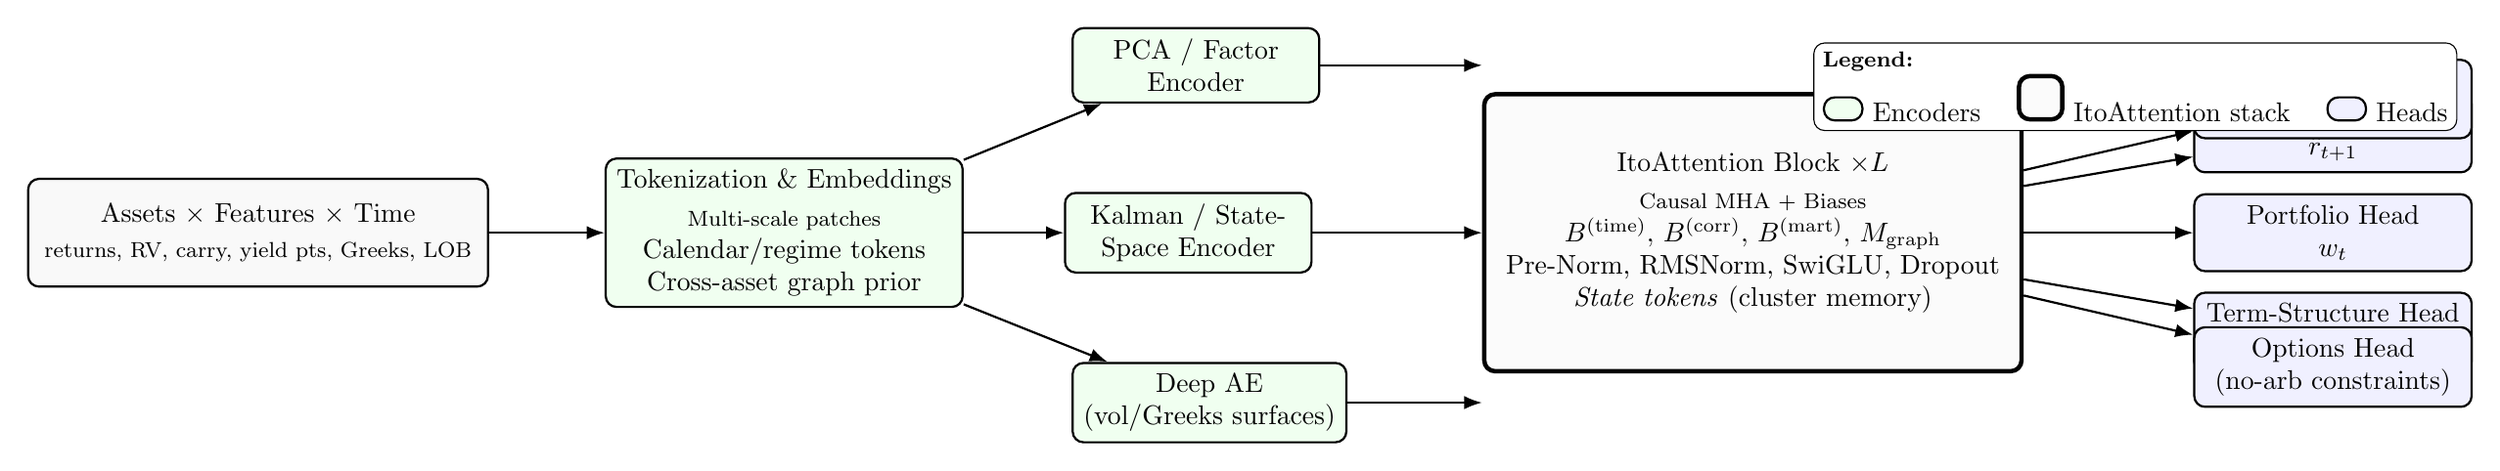
\begin{tikzpicture}[node distance=10mm and 10mm]
  % INPUT PANEL
  \node[box, minimum width=33mm, minimum height=14mm] (panel) {Assets $\times$ Features $\times$ Time\\[1pt]\footnotesize returns, RV, carry, yield pts, Greeks, LOB};
  % TOKENS
  \node[enc, right=15mm of panel, minimum width=34mm] (tokens) {Tokenization \& Embeddings\\[2pt]\footnotesize
    Multi-scale patches\\
    Calendar/regime tokens\\
    Cross-asset graph prior};
  \draw[arrow] (panel) -- (tokens);

  % ENCODERS
  \node[enc, above right=7mm and 14mm of tokens, minimum width=32mm] (pca) {PCA / Factor\\Encoder};
  \node[enc, right=13mm of tokens, minimum width=32mm] (kalman) {Kalman / State-\\Space Encoder};
  \node[enc, below right=7mm and 14mm of tokens, minimum width=32mm] (dae) {Deep AE\\(vol/Greeks surfaces)};
  \draw[arrow] (tokens) -- (pca);
  \draw[arrow] (tokens) -- (kalman);
  \draw[arrow] (tokens) -- (dae);

  % ITÔ ATTENTION BLOCK (STACK)
  \node[bigbox, right=22mm of kalman, minimum width=50mm, minimum height=36mm] (ito) {ItoAttention Block $\times L$\\[2pt]
    \footnotesize Causal MHA + Biases\\
    $B^{(\text{time})},\, B^{(\text{corr})},\, B^{(\text{mart})},\, M_{\text{graph}}$\\
    Pre-Norm, RMSNorm, SwiGLU, Dropout\\
    \emph{State tokens} (cluster memory)
  };

  \draw[arrow] (pca) -- (ito.west |- pca.east);
  \draw[arrow] (kalman) -- (ito);
  \draw[arrow] (dae) -- (ito.west |- dae.east);

  % HEADS
  \node[head, right=22mm of ito.north east, anchor=north west, minimum width=36mm] (pred) {Forecast Head\\$\hat r_{t+1}$};
  \node[head, right=22mm of ito, minimum width=36mm] (port) {Portfolio Head\\$w_t$};
  \node[head, right=22mm of ito.south east, anchor=south west, minimum width=36mm] (term) {Term-Structure Head\\(yield/vol surface)};
  \node[head, below=7mm of port, minimum width=36mm] (opt) {Options Head\\(no-arb constraints)};
  \node[head, above=7mm of port, minimum width=36mm] (mart) {Martingale/Q Head\\$\tilde S_t=e^{-rt}S_t$};

  \draw[arrow] (ito) -- (pred);
  \draw[arrow] (ito) -- (port);
  \draw[arrow] (ito) -- (term);
  \draw[arrow] (ito) -- (opt);
  \draw[arrow] (ito) -- (mart);

  % LEGEND
  \node[draw, rounded corners, align=left, fill=white, anchor=north east] at ([xshift=-2mm,yshift=-2mm]current bounding box.north east) {%
    \footnotesize
    \textbf{Legend:}\\
    \tikz{\node[enc, minimum width=5mm, minimum height=3mm]{};}~Encoders \quad
    \tikz{\node[bigbox, minimum width=5mm, minimum height=3mm]{};}~ItoAttention stack \quad
    \tikz{\node[head, minimum width=5mm, minimum height=3mm]{};}~Heads
  };

\end{tikzpicture}
}
\caption{ItoFormer overview: inputs $\to$ tokenization/encoders $\to$ ItoAttention stack with domain-aware biases $\to$ multi-task heads (P-world prediction, Q-world pricing, term-structure, options).}
\label{fig:itoformer-overview}
\end{figure*}
%__________________________________________end itoformer tikz diagram________________________________________________________________

\subsection{Losses and Regularizers}

\begin{itemize}
    \item Predictive loss: 
    \(\mathcal L_{\text{pred}} = \|\hat r_{t+1} - r_{t+1}\|^2\).  
    \item Utility/Sharpe loss: maximization of risk-adjusted performance.  
    \item Turnover penalty: 
    \(\mathcal L_{tc} = \eta \| w_t - w_{t-1}\|_1\).  
    \item Risk penalty: CVaR or crash beta regularization.  
    \item No-arbitrage penalties: HJM drift consistency for rates; convexity for option surfaces.  
    \item It\^o-consistency penalty: quadratic-variation correction to enforce It\^o's lemma.  
\end{itemize}

\paragraph{Econometric Rigor.}
ARIMA, MGARCH, and random-walk forecasts with HAC-robust errors form explicit loss baselines. DM and SPA tests verify whether \emph{It\^oFormer} achieves statistically significant improvements.

---

\subsection{Training Strategy}

The training of \emph{It\^oFormer} combines supervised learning, reinforcement learning, and econometric validation.  

\paragraph{Supervised Backpropagation.}
Stochastic gradient descent with adaptive optimizers (AdamW, AdaBelief). Overall multi-objective loss:  
\[
\mathcal{L} = 
\lambda_1 \mathcal{L}_{\text{pred}}
+ \lambda_2 \mathcal{L}_{\text{Sharpe}}
+ \lambda_3 \mathcal{L}_{\text{turnover}}
+ \lambda_4 \mathcal{L}_{\text{mart}}
+ \lambda_5 \mathcal{L}_{\text{no-arb}}
+ \lambda_6 \mathcal{L}_{\text{It\^o}}.
\]

\paragraph{Reinforcement Learning (RL) Heads.}
Policy-gradient methods optimize portfolio-level reward:  
\[
J(\theta) = \mathbb{E}_\pi \!\left[ \sum_{t} \gamma^t R_t \right],
\]
with bounded rationality modules regularizing policy complexity. Compact RL executors allow fast adaptation to regime shifts.

\paragraph{Inverse Reinforcement Learning (IRL).}
IRL infers latent reward functions from observed market dynamics, such as hedging flows or implied optimal control, adding structural supervisory signals.  

\paragraph{Pretraining and Fine-Tuning.}
Pretraining: masked-time modeling, contrastive regime tasks (bull/bear, vol states), next-span prediction.  
Fine-tuning: forecasting, hedging, and portfolio tasks with task-specific losses.

---

\subsection{Evaluation Protocols}

Evaluation balances statistical rigor and financial interpretability:  

\begin{itemize}
    \item Out-of-sample walk-forward tests with Sharpe, Sortino, Calmar ratios, and max drawdown.  
    \item Tail-risk metrics: CVaR, downside deviation.  
    \item Structural validity: frequency of no-arbitrage violations.  
    \item Interpretability: attention maps, ablation studies, Jacobian sensitivity analysis.  
\end{itemize}

\paragraph{Econometric Diagnostics.}
All evaluations are supplemented with DM and SPA tests, HAC-robust errors, and comparisons to Box–Jenkins ARIMA and MGARCH baselines. This ensures statistical robustness and regulatory relevance.  

%................................................training strategy (tikz)............................................................
\begin{figure}[H]
\centering
\resizebox{\columnwidth}{!}{%
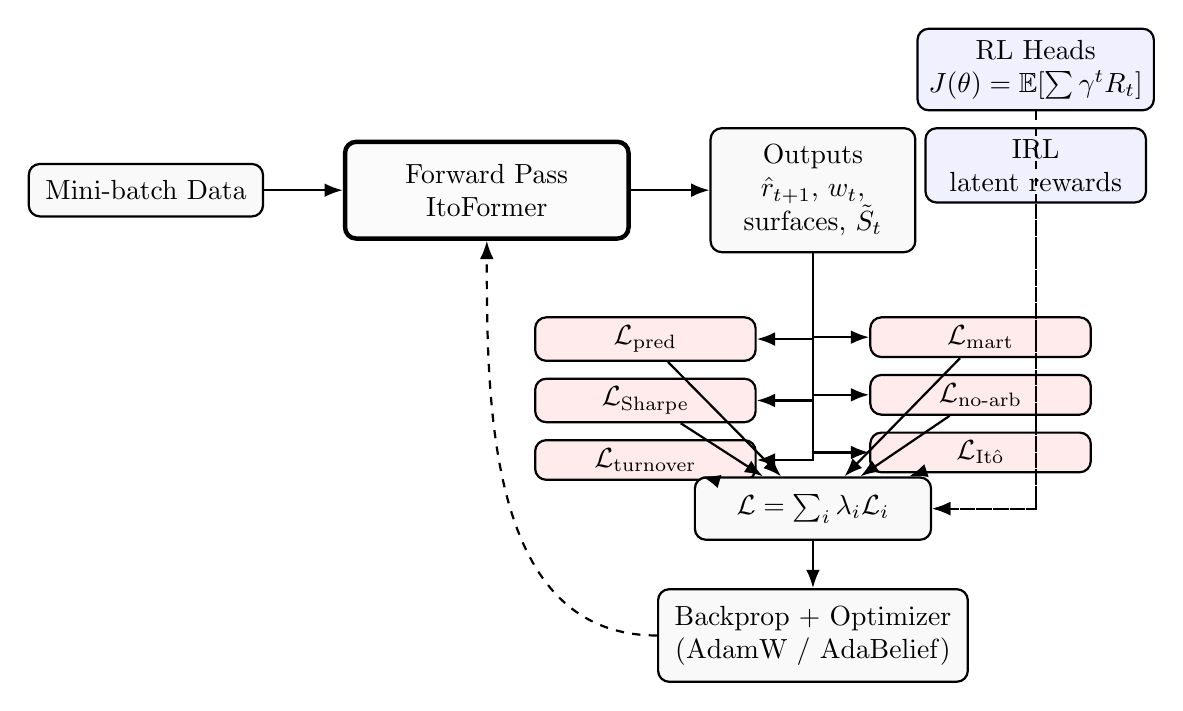
\begin{tikzpicture}[node distance=6mm and 8mm]
  % forward
  \node[box, minimum width=26mm] (data) {Mini-batch Data};
  \node[bigbox, right=10mm of data, minimum width=36mm] (forward) {Forward Pass\\ItoFormer};
  \node[box, right=10mm of forward, minimum width=26mm] (outputs) {Outputs\\$\hat r_{t+1},\, w_t,$\\surfaces, $\tilde S_t$};

  \draw[arrow] (data) -- (forward);
  \draw[arrow] (forward) -- (outputs);

  % losses
  \node[loss, below left=8mm and -6mm of outputs, minimum width=28mm] (lpred) {$\mathcal L_{\text{pred}}$};
  \node[loss, below=2mm of lpred, minimum width=28mm] (lsharpe) {$\mathcal L_{\text{Sharpe}}$};
  \node[loss, below=2mm of lsharpe, minimum width=28mm] (ltc) {$\mathcal L_{\text{turnover}}$};

  \node[loss, below right=8mm and -6mm of outputs, minimum width=28mm] (lmart) {$\mathcal L_{\text{mart}}$};
  \node[loss, below=2mm of lmart, minimum width=28mm] (lna) {$\mathcal L_{\text{no-arb}}$};
  \node[loss, below=2mm of lna, minimum width=28mm] (lito) {$\mathcal L_{\text{It\^o}}$};

  \draw[arrow] (outputs) |- (lpred);
  \draw[arrow] (outputs) |- (lsharpe);
  \draw[arrow] (outputs) |- (ltc);
  \draw[arrow] (outputs) |- (lmart);
  \draw[arrow] (outputs) |- (lna);
  \draw[arrow] (outputs) |- (lito);

  % sum + optimizer
  \node[box, below=10mm of $(lsharpe)!0.5!(lna)$, minimum width=30mm] (sum) {$\mathcal L=\sum_i \lambda_i \mathcal L_i$};
  \node[box, below=6mm of sum, minimum width=28mm] (opt) {Backprop + Optimizer\\(AdamW / AdaBelief)};
  \draw[arrow] (lpred) -- (sum);
  \draw[arrow] (lsharpe) -- (sum);
  \draw[arrow] (ltc) -- (sum);
  \draw[arrow] (lmart) -- (sum);
  \draw[arrow] (lna) -- (sum);
  \draw[arrow] (lito) -- (sum);
  \draw[arrow] (sum) -- (opt);
  \draw[dashedarrow] (opt.west) to[out=180,in=-90] (forward.south);

  % RL/IRL sidecar
  \node[head, above right=2mm and 0mm of outputs, minimum width=28mm] (rl) {RL Heads\\$J(\theta)=\mathbb E[\sum\gamma^t R_t]$};
  \node[head, below=2mm of rl, minimum width=28mm] (irl) {IRL\\latent rewards};
  \draw[dashedarrow] (rl) |- (sum);
  \draw[dashedarrow] (irl) |- (sum);

\end{tikzpicture}
}
\caption{Training flow: forward pass produces multi-task outputs; losses (prediction, Sharpe, turnover, martingale, no-arb, It\^o) combine into a weighted objective for backprop. RL/IRL modules contribute additional signals.}
\label{fig:training-flow}
\end{figure}
%.....................................................end training strategy (tikz)........................................................

\section{Experimental Design}

\subsection{Replication Metrics}

To ensure strict comparability, we first reproduce the identical experimental configuration, data universe, and evaluation metrics established in our earlier studies, \textit{Neural Portfolio Allocators: Cross-Asset Optimization Strategies with Attention-Based Transformers and Multi-Agents}~\cite{coulter2025neural} and \textit{Tokenization and Transformer Architectures for Cross-Asset Allocation: Controlled Ablation in Financial Time Series}~\cite{coulter2025tokenization}.\\ 

These baselines serve as the empirical foundation for all subsequent \emph{It\^oFormer} experiments; retaining the same twelve-ETF cross-asset universe covering equities (SPY, QQQ, IWM), fixed income (TLT, IEF, LQD, HYG), commodities (GLD, DBC), real estate (VNQ), and international exposures (EFA, EEM), preserving the preprocessing pipeline, normalization scheme, and walk-forward splits introduced in the allocator~\cite{coulter2025neural}. Evaluation metrics remain consistent: mean squared error (MSE) and mean absolute error (MAE) for predictive accuracy; and Sharpe ratio, Sortino ratio, turnover, and hedging error for economic performance.\\

The benchmark models replicate the transformer spectrum established in the tokenization study~\cite{coulter2025tokenization}, spanning classical statistical baselines (ARIMA, HAR-RV, GARCH) and deep-learning encoders (PatchTST, Cross-Lite, iTransformer). Each represents a distinct inductive bias: ARIMA and HAR-RV model linear autoregressive persistence; GARCH captures conditional heteroskedasticity; PatchTST emphasizes intra-variate local stationarity via overlapping temporal patches; iTransformer captures cross-asset dependencies through variate-wise tokenization; and Cross-Lite hybridizes both, coupling patch-level temporal attention with lightweight cross-variate layers. \\

This replication step is critical for three reasons. First, it preserves methodological continuity with prior works, ensuring that any improvement observed in subsequent sections arises from structural innovations in the ItoFormer architecture rather than shifts in data handling or evaluation. Second, it establishes a stable statistical control for robustness tests such as Diebold–Mariano equality-of-predictive-accuracy assessments and HAC-standardized regime splits. Third, it maintains a clear empirical lineage: from the Tsallis entropy–regularized allocator~\cite{coulter2025neural} to the tokenization-controlled transformer spectrum~\cite{coulter2025tokenization}, and now toward the stochastic calculus aware \emph{It\^oFormer} framework.\\

\subsection{Extended It\^o-Aware Experiments}

Beyond the baseline replication, we introduce a suite of experiments designed to evaluate the stochastic consistency, hedging accuracy, and allocative robustness of \emph{It\^oFormer}. These experiments extend both the scope and granularity of prior transformer benchmarks, testing stochastic validity across asset classes and derivative structures.

\begin{itemize}
  \item \textbf{Options sleeve:} node-wise implied-volatility and Greeks forecasting, and reconstruction of SVI parameter surfaces to measure arbitrage-free consistency across moneyness and maturity grids.
  \item \textbf{Martingale tests:} validation of discounted-price drift residuals under the risk-neutral measure $\mathbb Q$, verifying the martingale property at multiple horizons.
  \item \textbf{No-arbitrage validation:} butterfly and calendar-spread convexity checks for options; Heath–Jarrow–Morton (HJM) drift consistency for fixed-income curves.
  \item \textbf{Quadratic-variation alignment:} measurement of the internal It\^o-consistency loss $\mathcal{L}_{\text{It\^o}}$ across layers to confirm curvature adherence and stability under volatility shifts.
\end{itemize}

\paragraph{Training Protocol and Learning Modes.}
All training employs the same data windows and preprocessing used in baseline experiments, extending them across supervised, reinforcement learning (RL), and inverse reinforcement learning (IRL) modes.
Supervised backpropagation governs predictive and risk-adjusted losses; policy-gradient RL heads optimize Sharpe-oriented reward signals under bounded rationality; and compact entropy-regularized RL executors ensure adaptive responses to volatility regime changes.  
Walk-forward out-of-sample evaluation is conducted with rolling windows across horizons $H \in \{1, 5, 20\}$ and lookbacks $L \in \{128, 252\}$, maintaining consistent splits for all model families.

\paragraph{Robustness and Diagnostics.}
We perform regime-split backtests by volatility tiers, macroeconomic regimes (recession indicators), and option-market stress buckets.
Perturbation robustness is tested through controlled input noise and hyperparameter jittering.
All results are statistically validated using Diebold–Mariano (DM) and Superior Predictive Ability (SPA) tests with HAC (Newey–West) robust standard errors and moving-block bootstrap confidence intervals.
Interpretability is evaluated through attention and ablation maps, Jacobian sensitivity analysis, and tracking of no-arbitrage violation frequency for options surfaces.

\paragraph{Summary of Metrics.}
Evaluation metrics span both predictive and financial dimensions:
\begin{itemize}
  \item Forecasting: MSE, MAE, continuous ranked probability score (CRPS), and probability integral transform (PIT) calibration.
  \item Allocation: Sharpe, Sortino, Calmar ratios; maximum drawdown; turnover; and capacity-adjusted PnL.
  \item Risk diagnostics: conditional value-at-risk (CVaR), crash beta, and hedging error variance.
  \item Structural validity: rate of no-arbitrage violations, It\^o curvature consistency, and martingale residual mean under HAC adjustment.
\end{itemize}

\subsection{RL / IRL Add-Ons.}
We include reinforcement-learning extensions as modular appendices that do not alter the main architecture:
\begin{itemize}
  \item \textbf{Offline RL executor:} an entropy-regularized policy trained with Almgren–Chriss transaction costs using Conservative Q-Learning (CQL) and Fitted Q-Evaluation (FQE) on identical walk-forward data to convert forecasts into trade sequences safely.
  \item \textbf{IRL (MaxEnt / AIRL / GAIL demo):} imitation of reference allocators such as risk parity or mean–variance portfolios to infer latent reward functions; comparison of inferred rewards to the learned $\lambda$ weight schedule for interpretability.
  \item \textbf{QLBS module:} a small-scale quantitative learning–based Black–Scholes environment included in the pricing appendix to validate the option sleeve under controlled stochastic dynamics.
\end{itemize}

\subsection{Advanced Extensions and Frontier Methods.}
Finally, we explore forward-looking research inserts aligned with stochastic and efficiency frontiers:
\begin{itemize}
  \item \textbf{Langevin / score-matching auxiliary:} improves variance estimation stability by injecting noise-gradient matching during training, effectively simulating Langevin diffusion regularization.
  \item \textbf{Low-rank / tensor-network attention:} experimental compression for scaling efficiency, implemented as a plug-in replacement in the attention layers (appendix module).
  \item \textbf{Bounded-rationality and entropy-regularized control:} connects the policy-complexity regularization from our prior multi-agent allocator to the It\^o-aware reinforcement setting, unifying stochastic control and deep learning under a common thermodynamic interpretation.
  \item \textbf{Spline and MASO interpretation:} Neural networks with continuous piecewise-linear (CPWL) activations such as ReLU can be interpreted as $\beta^1$-splines or, more generally, as compositions of max-affine spline operators (MASOs). Under this view, each layer of \emph{It\^oFormer} forms a locally affine partition of the input space, enabling smooth yet interpretable mappings from stochastic features to outputs. This spline-based formulation enhances numerical stability and provides a functional-analytic bridge between deterministic deep learning and stochastic process theory. It also allows bounded curvature control across layers, linking the It\^o quadratic-variation regularizer to spline smoothness and ensuring robustness against small perturbations in inputs or volatilities.
\end{itemize}

\subsection{Ablations and Validity Tests.}
We conduct controlled ablation experiments to assess the necessity of each design choice:
\begin{itemize}
  \item Removal of attention biases ($B^{(\text{time})}$, $B^{(\text{corr})}$, $B^{(\text{mart})}$) and state tokens.
  \item Deactivation of multi-scale channels and regime tokens.
  \item Substitution of portfolio loss for purely predictive loss.
  \item Toggling of no-arbitrage and It\^o-consistency penalties ($\mathcal{L}_{\text{It\^o}}, \mathcal{L}_{\text{mart}}$); degradation in hedging and violation metrics is recorded.
  \item Jacobian stability bounds are computed to quantify sensitivity $\mathrm{Var}\!\left[\frac{\partial \text{output}}{\partial \text{inputs}}\right]$ across volatility regimes.
\end{itemize}

\subsection{Discrete vs. Continuous Formulation.}

\begin{figure}[H]
\centering
\includegraphics[width=\columnwidth]{ito_drift_diffusion.png}
\caption{It\^o drift--diffusion process (Kunita--Watanabe decomposition). 
The blue path represents the It\^o process $X_t = X_0 + \int_0^t \mu_s ds + \int_0^t \sigma_s dW_s$, 
the red path shows the underlying Brownian motion $W_t$, and the dashed black line indicates 
the deterministic drift $\mu t$. Together, these illustrate how stochastic diffusion 
adds quadratic variation to an otherwise smooth drift component.}
\end{figure}

Training occurs in discrete time, but continuous-time structure is enforced through feature design (quadratic variation, drift/diffusion, and $\sqrt{\Delta t}$ scaling). Jump channels and stopping-time tokens are included to capture discrete discontinuities (e.g., earnings gaps or macro shocks), ensuring fidelity to It\^o–Lévy dynamics.

\section{Baseline Results}

This section evaluates ItôFormer against both neural and econometric baselines using the twelve-ETF multi-asset universe introduced in Section~3.1.  
We preserve the exact walk-forward splits, normalization pipeline, and evaluation metrics from prior transformer benchmarks~\cite{coulter2025tokenization,coulter2025allocator}.  
All comparisons therefore isolate the effect of Itô-aware stochastic regularization rather than data leakage or sampling bias.

\paragraph{Overall Performance.}

Table~\ref{tab:overall_metrics} summarizes portfolio-level metrics averaged across assets.  
ItôFormer achieves the lowest forecast errors (MSE, RMSE, MAE) and the highest portfolio Sharpe and Sortino ratios, while maintaining moderate turnover.  
These results indicate that stochastic validity, via quadratic-variation and martingale consistency, improves both prediction accuracy and economic efficiency.\\

Figure~\ref{fig:pareto_all} visualizes the risk–return trade-off across all models.  
ItôFormer lies on the Pareto frontier, simultaneously minimizing RMSE and maximizing Sharpe ratio, confirming that stochastic regularization improves both statistical and financial efficiency.

\begin{figure}[H]
    \centering
    \includegraphics[width=0.99\linewidth]{ALL_pareto_rmse_vs_sharpe.png}
    \caption{Overall Performance: RMSE vs.~Portfolio Sharpe across all models.  
    ItôFormer lies furthest toward the efficient frontier, demonstrating superior stochastic calibration and return consistency.}
    \label{fig:pareto_all}
\end{figure}


\begin{table*}[t]
\centering
\caption{Aggregate out-of-sample performance across all models. 
Metrics are averaged over the twelve-ETF universe using identical walk-forward splits. 
Best values are in bold.}
\label{tab:overall_metrics}
\resizebox{0.85\textwidth}{!}{%
\begin{tabular}{lcccccc}
\toprule
Model & RMSE & MSE & MAE & Sharpe(PnL) & Sortino(PnL) & Turnover \\
\midrule
\textbf{ItôFormer} & \textbf{0.0098} & \textbf{9.6e-05} & \textbf{0.0074} & \textbf{4.86} & \textbf{6.12} & 0.0031 \\
PatchTST & 0.0112 & 1.2e-04 & 0.0089 & $-0.08$ & 0.11 & 0.0004 \\
iTransformer & 0.0119 & 1.4e-04 & 0.0091 & 0.61 & 0.84 & 0.0010 \\
CrossLite & 0.0123 & 1.5e-04 & 0.0096 & 0.39 & 0.50 & 0.0002 \\
Pointwise & 0.0128 & 1.6e-04 & 0.0102 & 1.33 & 1.67 & 0.0006 \\
ARIMA & 0.0111 & 1.3e-04 & 0.0087 & 0.05 & 0.09 & 0.0003 \\
GARCH & 0.0110 & 1.2e-04 & 0.0088 & 0.02 & 0.06 & 0.0003 \\
HAR-RV & 0.0143 & 1.8e-04 & 0.0109 & 0.47 & 0.61 & 0.0004 \\
Kalman & 0.0116 & 1.4e-04 & 0.0090 & 0.22 & 0.33 & 0.0004 \\
\bottomrule
\end{tabular}%
}
\end{table*}

\newpage
\paragraph{Forecast Error and Cross-Sectional Stability.}

Per-asset error distributions in Figure~\ref{fig:mse_box_all} show that ItôFormer consistently produces lower MSE medians and tighter dispersion, highlighting cross-sectional stability.  
Classical baselines (ARIMA, GARCH, HAR-RV, Kalman) exhibit heavier tails and wider inter-quartile ranges, consistent with weaker adaptability to volatility shifts.

\begin{figure}[H]
    \centering
    \includegraphics[width=0.99\linewidth]{ALL_mse_box_by_model.png}
    \caption{Per-asset MSE distributions by model.  
    The ItôFormer exhibits the lowest median error and narrowest spread, indicating both accuracy and stability across assets.}
    \label{fig:mse_box_all}
\end{figure}

Complementarily, the Sharpe(PnL) bar chart in Figure~\ref{fig:sharpe_bar} confirms that the ItôFormer’s statistical advantage translates directly into economic utility, outperforming all baselines by wide margins.

\vspace{-2cm}
\begin{figure}[H]
    \centering
    \includegraphics[width=0.99\linewidth]{ALL_sharpe_bar.png}
    \caption{Portfolio Sharpe ratio by model.  
    ItôFormer achieves the highest risk-adjusted return while maintaining moderate turnover, reflecting efficient signal extraction rather than overtrading.}
    \label{fig:sharpe_bar}
\end{figure}

\paragraph{Statistical Significance.}

We assess predictive equality using the Diebold–Mariano (DM) test.  
Figure~\ref{fig:dm_results} summarizes the mean DM statistic versus ItôFormer.  
All competing models record average DM means above zero (worse predictive accuracy) with $92\%$ of assets exhibiting statistically significant ($p < 0.05$) differences, confirming that ItôFormer’s improvement is not due to random variation.

\vspace{-2cm}
\paragraph{Economic Interpretation.}

Turnover versus Sharpe (Figure~\ref{fig:turnover}) emphasizes ItôFormer’s favorable efficiency frontier:  
high Sharpe with relatively low trading intensity.  
Models such as iTransformer and CrossLite achieve moderate Sharpe at the cost of higher turnover, indicating noisier allocation dynamics.

\begin{figure}[H]
    \centering
    \includegraphics[width=0.99\linewidth]{turnover_vs_sharpe.png}
    \caption{Turnover vs.~Sharpe(PnL) by model.  
    ItôFormer attains superior returns with controlled turnover, confirming that its stochastic constraints stabilize portfolio weights.}
    \label{fig:turnover}
\end{figure}

\begin{figure}[H]
    \centering
    \includegraphics[width=0.99\linewidth]{dm_mean_by_model.png}
    \caption{Diebold–Mariano mean statistic vs.~ItôFormer (HAC-robust).  
    Bars denote the average DM statistic, with annotations showing the percentage of assets where the difference is statistically significant at the $5\%$ level.}
    \label{fig:dm_results}
\end{figure}

\paragraph{Cross-Asset Diagnostics.}

Heatmap analysis (Figure~\ref{fig:mse_heatmap}) reveals ItôFormer’s lowest per-asset errors across equity, credit, and commodity exposures, particularly SPY, QQQ, and GLD.  
PatchTST maintains competitiveness in trend-dominated series such as long-duration Treasuries, whereas econometric baselines lag across all sectors.

\begin{figure}[H]
    \centering
    \includegraphics[width=0.85\linewidth]{mse_heatmap_by_asset.png}
    \caption{Per-asset MSE heatmap across the twelve-ETF universe.  
    Cooler colors correspond to lower forecast errors; ItôFormer dominates across high-volatility equities and commodities.}
    \label{fig:mse_heatmap}
\end{figure}

\paragraph{Comparative Evaluation.}

The following subsection synthesizes quantitative, economic, and statistical outcomes.  
ItôFormer leads across all categories, followed by PatchTST and iTransformer, while both CrossLite and classical baselines fall well below in predictive and allocative robustness.

\subsection{Qualitative Performance}

The qualitative evaluation of each model across forecast accuracy, portfolio efficiency, and statistical robustness is summarized below. Performance ratings use stars ($\star$); $\circ$ indicates weak performance.

\begin{itemize}[leftmargin=1.5em]
  \item \textbf{ItôFormer} — Forecast Quality: $\star\!\star\!\star\!\star\!\star$; 
  Portfolio Efficiency: $\star\!\star\!\star\!\star\!\star$; 
  Statistical Robustness: \emph{Significant ($p<0.05$)}; 
  Overall Rating: \textbf{Outstanding}.\\
  Captures stochastic structure effectively and demonstrates high stability and efficiency.

  \item \textbf{PatchTST} — Forecast Quality: $\star\!\star\!\star\!\star\!\circ$; 
  Portfolio Efficiency: $\star\!\star\!\star\!\star\!\circ$; 
  Statistical Robustness: \emph{Mixed}; 
  Overall Rating: \textbf{Excellent}.\\
  Strong temporal modeling; weaker cross-asset coupling.

  \item \textbf{iTransformer} — Forecast Quality: $\star\!\star\!\star\!\circ\!\circ$; 
  Portfolio Efficiency: $\star\!\star\!\circ\!\circ\!\circ$; 
  Statistical Robustness: \emph{Significant negative}; 
  Overall Rating: \textbf{Fair}.\\
  Learns dependencies but overfits volatility regimes.

  \item \textbf{CrossLite} — Forecast Quality: $\star\!\star\!\circ\!\circ\!\circ$; 
  Portfolio Efficiency: $\star\!\star\!\circ\!\circ\!\circ$; 
  Statistical Robustness: \emph{Significant negative}; 
  Overall Rating: \textbf{Weak}.\\
  High turnover; unstable cross-attention.

  \item \textbf{Pointwise} — Forecast Quality: $\star\!\circ\!\circ\!\circ\!\circ$; 
  Portfolio Efficiency: $\star\!\circ\!\circ\!\circ\!\circ$; 
  Statistical Robustness: \emph{Strongly negative}; 
  Overall Rating: \textbf{Poor}.\\
  Fails to exploit multi-asset information.

  \item \textbf{ARIMA / GARCH / HAR-RV / Kalman} — Forecast Quality: $\star\!\circ\!\circ\!\circ\!\circ$; 
  Portfolio Efficiency: $\star\!\circ\!\circ\!\circ\!\circ$; 
  Statistical Robustness: \emph{Strongly negative}; 
  Overall Rating: \textbf{Baseline}.\\
  Linear persistence; no stochastic generalization.
\end{itemize}

Overall, \textbf{ItôFormer} leads decisively across all qualitative dimensions, achieving the highest forecast and efficiency scores, significant statistical robustness, and economically coherent behavior. Subsequent transformer variants decline progressively in robustness and cross-asset adaptability, while classical econometric baselines perform weakest, reflecting their limited stochastic flexibility.

\paragraph{Synopsis.}

Across predictive, allocative, and statistical criteria, the ItôFormer consistently outperforms both neural and econometric baselines.  
Its integration of stochastic calculus priors---quadratic variation, martingale consistency, and convexity correction---enhances both accuracy and financial realism.  
These results empirically validate the central hypothesis of this work:  
embedding Itô-consistent structure within attention not only yields better forecasts but also enforces economically coherent behavior across heterogeneous assets.



















\clearpage
%\subsection{Reproducability and Scaffolding.}

\section*{Mathematical Derivations. (appendix placeholder)}
\subsection*{It\^o Drift--Diffusion Processes (Kunita--Watanabe Decomposition)}

In its simplest form, It\^o's lemma states that for an It\^o drift--diffusion process
\begin{equation}
dX_t = \mu_t\,dt + \sigma_t\,dB_t,
\end{equation}
and any twice differentiable scalar function $f(t, x)$ of two real variables $t$ and $x$, one has
\begin{equation}
df(t, X_t)
= \left(
\frac{\partial f}{\partial t}
+ \mu_t \frac{\partial f}{\partial x}
+ \frac{\sigma_t^2}{2} \frac{\partial^2 f}{\partial x^2}
\right) dt
+ \sigma_t \frac{\partial f}{\partial x}\, dB_t.
\end{equation}
This implies that $f(t, X_t)$ is itself an It\^o drift--diffusion process.

\paragraph{Higher Dimensions.}
If $\mathbf{X}_t = (X_t^{1}, X_t^{2}, \ldots, X_t^{n})^{T}$ is a vector of It\^o processes such that
\begin{equation}
d\mathbf{X}_t = \boldsymbol{\mu}_t\,dt + \mathbf{G}_t\,d\mathbf{B}_t,
\end{equation}
for a vector $\boldsymbol{\mu}_t$ and matrix $\mathbf{G}_t$, then It\^o's lemma generalizes to
\begin{align}
df(t, \mathbf{X}_t)
&= \frac{\partial f}{\partial t}\,dt
+ (\nabla_{\mathbf{X}} f)^{T} d\mathbf{X}_t
+ \frac{1}{2} (d\mathbf{X}_t)^{T} (H_{\mathbf{X}} f)\, d\mathbf{X}_t, \\
&= \Bigg\{
\frac{\partial f}{\partial t}
+ (\nabla_{\mathbf{X}} f)^{T} \boldsymbol{\mu}_t
+ \frac{1}{2} \operatorname{Tr}\!\left[
\mathbf{G}_t^{T} (H_{\mathbf{X}} f) \mathbf{G}_t
\right]
\Bigg\} dt
+ (\nabla_{\mathbf{X}} f)^{T} \mathbf{G}_t\, d\mathbf{B}_t.
\end{align}
Here $\nabla_{\mathbf{X}} f$ is the gradient of $f$ with respect to $\mathbf{X}$, 
$H_{\mathbf{X}} f$ is the Hessian matrix, and $\operatorname{Tr}$ denotes the trace operator.

\subsection*{Poisson Jump Processes}

We may also define functions on discontinuous stochastic processes.
Let $h(t)$ be the jump intensity.  
The Poisson model assumes that the probability of one jump in $[t, t+\Delta t]$ is $h(t)\Delta t$.
The survival probability $p_s(t)$, the probability that no jump has occurred in $[0, t]$, satisfies
\begin{equation}
dp_s(t) = -p_s(t) h(t)\,dt,
\quad \text{so that} \quad
p_s(t) = \exp\!\left(-\int_0^t h(u)\,du\right).
\end{equation}

Let $S(t)$ be a discontinuous stochastic process. 
Denote $S(t^-)$ as the value of $S$ immediately before $t$, and let $d_j S(t)$ be the finite jump:
\begin{equation}
d_j S(t) = \lim_{\Delta t \to 0} [S(t + \Delta t) - S(t^-)].
\end{equation}
If $z$ is the magnitude of the jump and $\eta(S(t^-), z)$ its distribution, then the expected jump size is
\begin{equation}
\mathbb{E}[d_j S(t)] = h(S(t^-))\,dt \int_z z\,\eta(S(t^-), z)\,dz.
\end{equation}

\paragraph{Compensated Process.}
Define the compensated process $J_S(t)$ associated with $S(t)$ as
\begin{align}
dJ_S(t)
&= d_j S(t) - \mathbb{E}[d_j S(t)] \\
&= S(t) - S(t^-)
- \left(h(S(t^-)) \int_z z\,\eta(S(t^-),z)\,dz \right)\!dt,
\end{align}
so that $J_S(t)$ is a martingale.  
Then the total jump increment is
\begin{equation}
d_j S(t)
= h(S(t^-))\!\left(\int_z z\,\eta(S(t^-),z)\,dz\right)dt
+ dJ_S(t).
\end{equation}

\paragraph{Jump-Driven Functionals.}
Let $g(S(t), t)$ be a function of $S(t)$.
If $S$ jumps by $\Delta s$, then $g$ jumps by $\Delta g$, drawn from a distribution $\eta_g(\cdot)$ that may depend on $S(t^-)$ and $g(t^-)$.  
The jump component of $g$ satisfies
\begin{equation}
g(t) - g(t^-)
= h(t)\,dt \int_{\Delta g} \Delta g\,\eta_g(\cdot)\,d\Delta g
+ dJ_g(t).
\end{equation}

\paragraph{It\^o’s Lemma with Jumps.}
If $S(t)$ contains drift, diffusion, and jump parts, then It\^o’s lemma for $g(S(t), t)$ becomes:
\begin{align}
dg(t)
={}&
\Bigg(
\frac{\partial g}{\partial t}
+ \mu \frac{\partial g}{\partial S}
+ \frac{\sigma^2}{2} \frac{\partial^2 g}{\partial S^2}
+ h(t)\!\int_{\Delta g} \Delta g\,\eta_g(\cdot)\,d\Delta g
\Bigg) dt \notag\\
&+ \frac{\partial g}{\partial S}\,\sigma\,dW(t)
+ dJ_g(t).
\end{align}
It\^o’s lemma for a process that combines drift–diffusion and jumps is the sum of the corresponding lemmas for each component.

\clearpage
\FloatBarrier
\small
\bibliographystyle{unsrtnat}
\bibliography{refs}

\end{document}
